% Created 2021-12-09 Thu 21:18
% Intended LaTeX compiler: pdflatex
\documentclass[11pt]{article}
\usepackage[utf8]{inputenc}
\usepackage[T1]{fontenc}
\usepackage{graphicx}
\usepackage{grffile}
\usepackage{longtable}
\usepackage{wrapfig}
\usepackage{rotating}
\usepackage[normalem]{ulem}
\usepackage{amsmath}
\usepackage{textcomp}
\usepackage{amssymb}
\usepackage{capt-of}
\usepackage{hyperref}
\author{Ali Kadum Hassan, Frederik Henriques Altmann, Gustav Emil Mark-Hansen}
\date{\today}
\title{Opg3}
\hypersetup{
 pdfauthor={Ali Kadum Hassan, Frederik Henriques Altmann, Gustav Emil Mark-Hansen},
 pdftitle={Opg3},
 pdfkeywords={},
 pdfsubject={},
 pdfcreator={Emacs 27.2 (Org mode 9.5)}, 
 pdflang={English}}
\begin{document}

\maketitle
\tableofcontents


\section{OPGAVE 1}
\label{sec:orgee43d00}

\subsection{a}
\label{sec:org707dbd0}
\begin{verbatim}
Hej
\end{verbatim}

\begin{center}
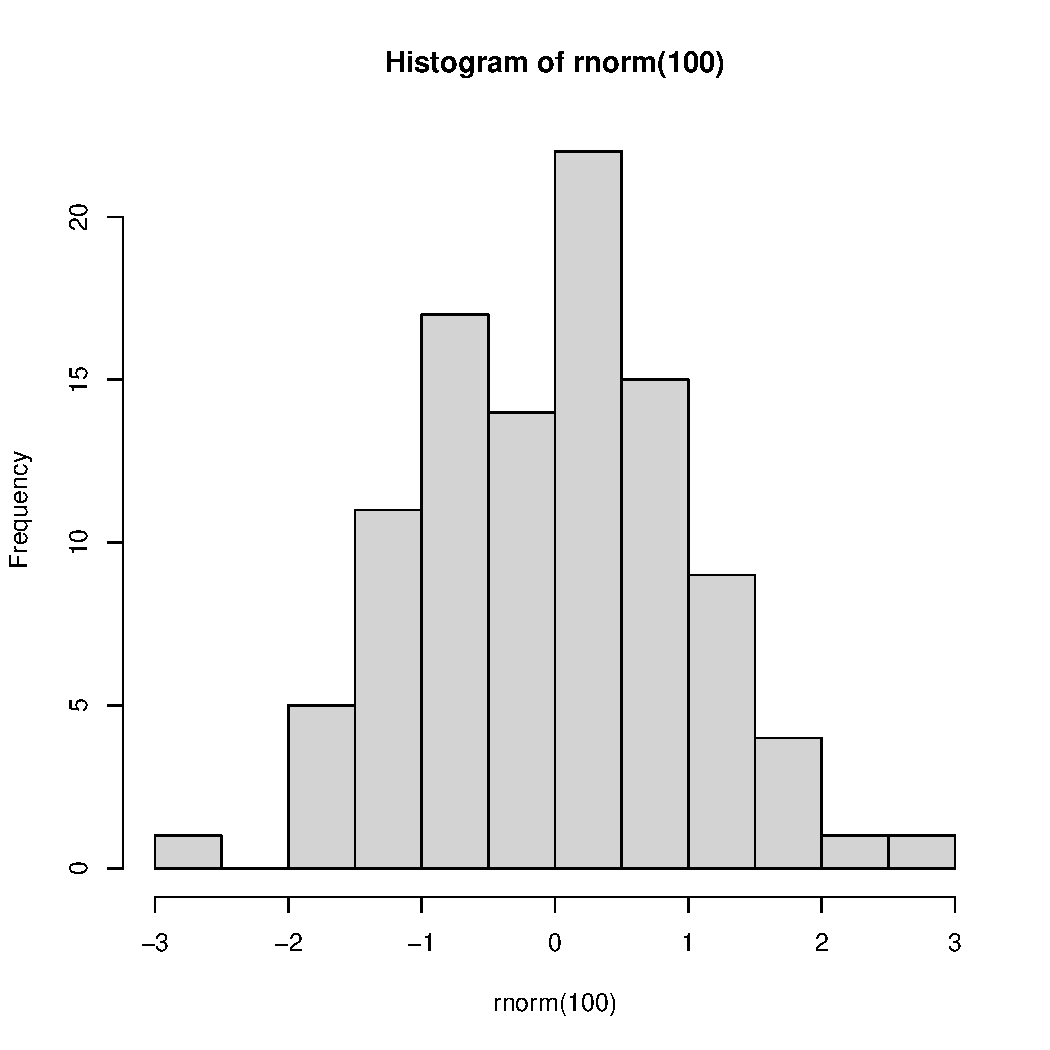
\includegraphics[width=.9\linewidth]{img.png}
\end{center}

Some text
\(e = mc^2\)

\subsection{a}
\label{sec:org07c1859}
Chancen for at få X kast der lander på krone i træk, er:
\((\frac{1}{2})^X\)

Skrevet i R:
\begin{verbatim}
pmf = \(throws) 0.5^throws
\end{verbatim}
\subsection{b}
\label{sec:org828cae8}
Profiten \(f(X)\) er givet ved \(f(a, X) = a2^X - a\)

Skrevet i R:
\begin{verbatim}
profit = \(buyin, throws) buyin * 2^(throws) - buyin
\end{verbatim}
\subsection{c}
\label{sec:orge8c304f}
\begin{align}
E(X) = \sum_{n=1}^\infty |f(b,n)|p(n) = \sum_{n=1}^\infty b \\
|f(x)|p(x) = b2^{x+1}0.5^x = b \\
\sum_{n=1}^\infty |f(b,n)|p(n) = \sum_{n=1}^\infty b = \infty
\end{align}

Da \(E(X)\) divergerer mod positiv uendelig har spillet ikke noget forventet udfald.
\section{2}
\label{sec:orgae2e124}
\subsection{a}
\label{sec:org2e4b348}
Da hele pmf \(p\), bortset fra \(p(x=-1,y=3)\) er kendt kan \(z\) beregnes ved at isolere.

\begin{center}
\begin{tabular}{lrrl}
p(x, y) & y = −1 & y = 1 & y = 3\\
x = −1 & 0.1 & 0.1 & z\\
x = 1 & 0.3 & 0.05 & 0.05\\
\end{tabular}
\end{center}

\begin{align}
\int p(x,y) &= 1 \\
1 &= 0.1 + 0.1 + 0.3 + 0.05 + 0.05 + z = 0.6 + z \\
z &= 1 - 0.6 = 0.4
\end{align}
\subsection{b}
\label{sec:orgacaf8ef}
\begin{align}
E[X+Y] &= E[X] + E[Y] \\
E[X] &= -1*0.6 + 1*0.4 = -0.2 \\
E[Y] &= -1*0.4 + 1*0.15 + 3*0.45 = 1.1 \\
E[X+Y] &= 1.1 - 0.2 = 0.9
\end{align}
\end{document}
